\documentclass[tikz,border=10pt]{standalone}

\begin{document}
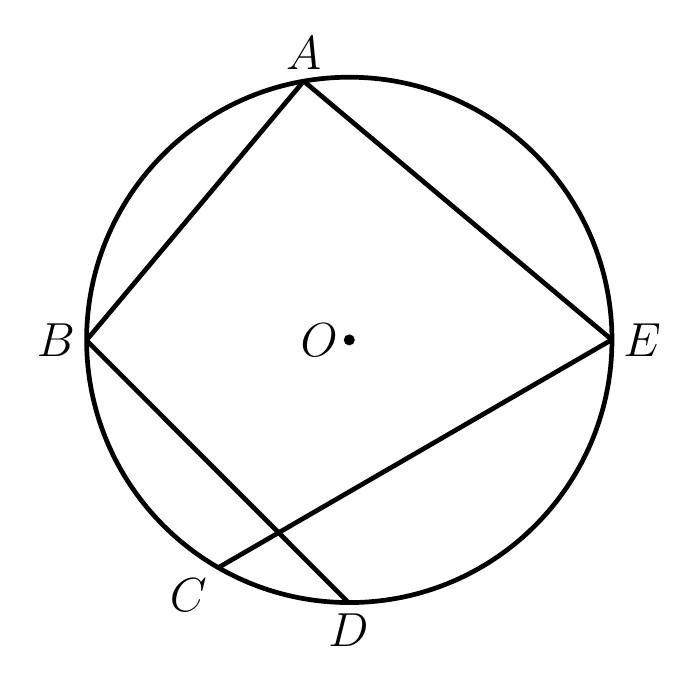
\begin{tikzpicture}[line width=1.7pt, line join=round, every node/.style={font=\fontsize{17}{20.4}\selectfont}]
\coordinate (A) at (-0.590,3.323);
\coordinate (B) at (-3.349,0.032);
\coordinate (C) at (-1.674,-2.855);
\coordinate (D) at (-0.022,-3.299);
\coordinate (O) at (-0.011,0.037);




\coordinate (E) at (3.323,0.039);


\draw (O) circle (3.336);


\draw (A) -- (B);
\draw (A) -- (E);
\draw (B) -- (D);
\draw (E) -- (C);


\fill (O) circle (0.070);


\node[above] at (A) {$A$};
\node[left] at (B) {$B$};
\node[below left] at (C) {$C$};
\node[below] at (D) {$D$};
\node[right] at (E) {$E$};
\node[left] at (O) {$O$};
\end{tikzpicture}
\end{document}